\section{ЗАДАНИЕ 1}

Составить диаграмму вычисления следующих выражений

\begin{lstlisting}
(equal 3 (abs (- 3)))
\end{lstlisting}

\begin{figure}[H]
    \centering
    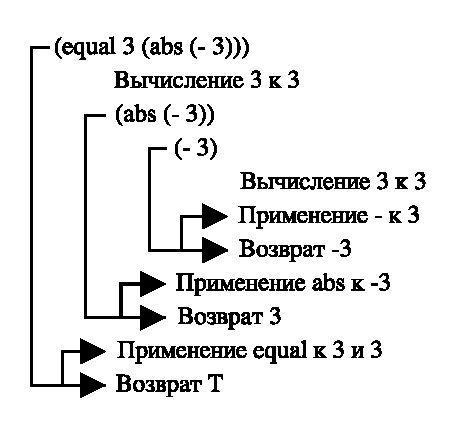
\includegraphics{img/01_01.pdf}
    \caption{Диаграмма для первого пункта}
\end{figure}

\begin{lstlisting}
(equal (+ 1 2) 3)
\end{lstlisting}

\begin{figure}[H]
    \centering
    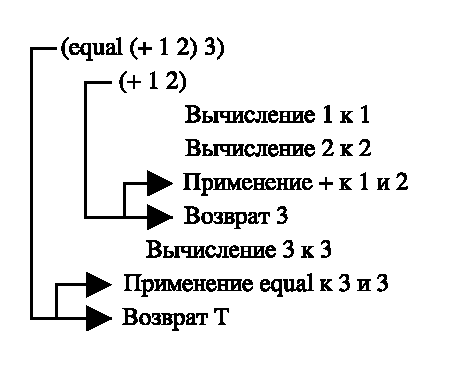
\includegraphics{img/01_02.pdf}
    \caption{Диаграмма для второго пункта}
\end{figure}

\begin{lstlisting}
(equal (* 4 7) 21)
\end{lstlisting}

\begin{figure}[H]
    \centering
    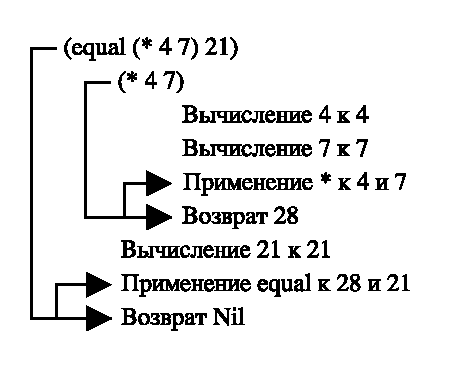
\includegraphics{img/01_03.pdf}
    \caption{Диаграмма для третьего пункта}
\end{figure}

\begin{lstlisting}
(equal (* 2 3) (+ 7 2))
\end{lstlisting}

\begin{figure}[H]
    \centering
    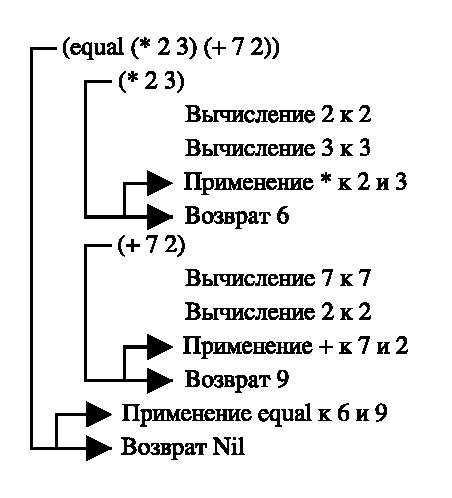
\includegraphics{img/01_04.pdf}
    \caption{Диаграмма для четвертого пункта}
\end{figure}

\begin{lstlisting}
(equal (- 7 3) (* 3 2))
\end{lstlisting}

\begin{figure}[H]
    \centering
    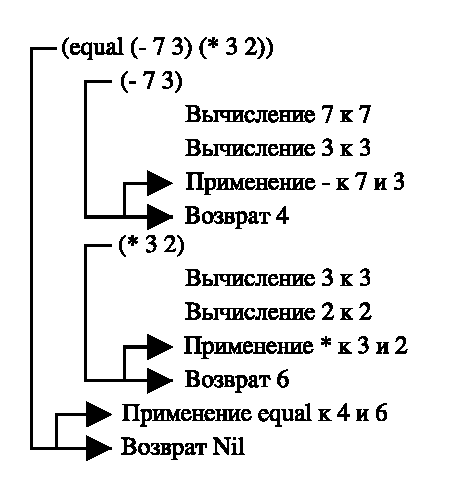
\includegraphics{img/01_05.pdf}
    \caption{Диаграмма для пятого пункта}
\end{figure}

\begin{lstlisting}
(equal (abs (- 2 4)) 3))
\end{lstlisting}

\begin{figure}[H]
    \centering
    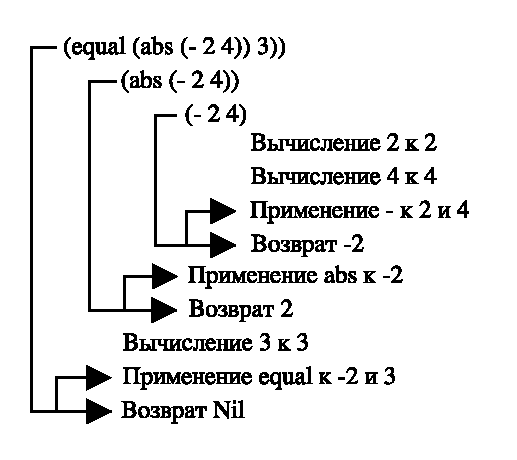
\includegraphics{img/01_06.pdf}
    \caption{Диаграмма для пятого пункта}
\end{figure}

\section{ЗАДАНИЕ 2}

Написать функцию, вычисляющую гипотенузу прямоугольного
треугольника по заданным катетам и составить диаграмму её вычисления.

\begin{lstlisting}
(defun hypotenuse (a b)
    (sqrt (+ (* a a) (* b b)))
)

(hypotenuse 4 3) ;;; 5.0
\end{lstlisting}

\begin{figure}[H]
    \centering
    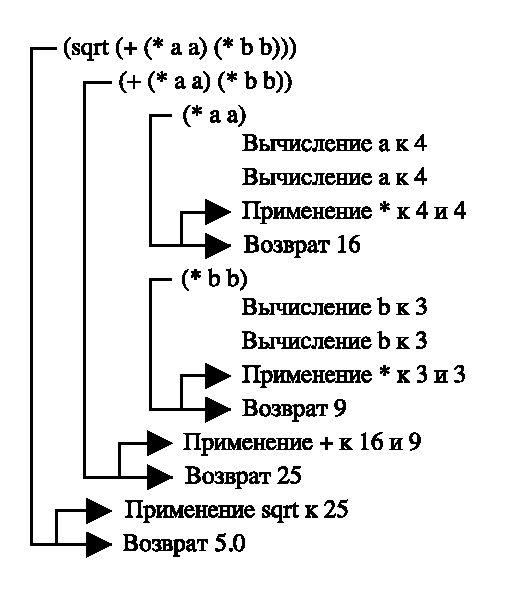
\includegraphics{img/02.pdf}
    \caption{Диаграмма для второго задания}
\end{figure}

\section{ЗАДАНИЕ 3}

Написать функцию, вычисляющую объем параллелепипеда
по 3-м его сторонам, и составить диаграмму ее вычисления.

\begin{lstlisting}
(defun volume (a b c)
    (* a b c)
)

(volume 2 3 4) ;;; 24
\end{lstlisting}

\begin{figure}[H]
    \centering
    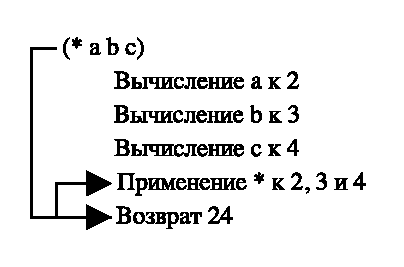
\includegraphics{img/03.pdf}
    \caption{Диаграмма для третьего задания}
\end{figure}

\section{ЗАДАНИЕ 4}

Каковы результаты вычисления следующих выражений

\begin{lstlisting}
(list 'a c)
;;; Результат: ошибка - нет переменной C

(cons'a (b c))
;;; Результат: ошибка - нет переменной C

(cons'a '(b c))
;;; Результат: (A B C)

(caddy (1 2 3 4 5))
;;; Результат: ошибка - нет функции CADDY

(cons'a'b'c)
;;; Результат: ошибка - неправильное количество аргументов
;;;(должно быть 2)

(list 'a (b c))
;;; Результат: ошибка - нет переменной C

(list a '(b c))
;;; Результат: ошибка - нет переменной A

(list (+ 1 '(length '(1 2 3))))
;;; Результат: ошибка - значение (LENGTH '(1 2 3)) не числовое
\end{lstlisting}

\section{ЗАДАНИЕ 5}

Написать функцию longer\_then от двух списков-аргументов,
которая возвращает Т, если первый аргумент имеет большую длину.

\begin{lstlisting}
(defun longer_then (list1 list2)
    (> (length list1) (length list2))
)

(longer_then '(1 2 3) '(1 2)) ;;; T
(longer_then '(1 2 3) '(1 2 3 4)) ;;; NIL
\end{lstlisting}

\section{ЗАДАНИЕ 6}

Каковы результаты вычисления следующих выражений?

\begin{lstlisting}
(cons 3 (list 5 6))
;;; Результат: (3 5 6)

(list 3 'from 9 'lives (- 9 3))
;;; Результат: (3 FROM 9 LIVES 6)

(+ (length for 2 too) (car '(21 22 23)))
;;; Результат: ошибка - нет переменной FOR

(cdr ' (cons is short for ans))
;;; Результат: (IS SHORT FOR ANS)

(car (list one two))
;;; Результат: ошибка - нет переменной ONE

(cons 3 '(list 5 6))
;;; Результат: (3 LIST 5 6)

(car (list 'one 'two))
;;; Результат: (ONE)
\end{lstlisting}
